\documentclass[12pt,a4paper,english]{article}
\usepackage{graphicx}
\usepackage[english]{babel}
\usepackage[utf8]{inputenc}
%\usepackage{listings}
\usepackage{multirow}
\usepackage{epstopdf}
\usepackage{amsmath}
\usepackage{amssymb}
\usepackage{mathpazo}
\usepackage{csquotes}
\usepackage{siunitx}
\usepackage{tikz}
\usepackage{booktabs}
\graphicspath{{./fig/}}

\setlength{\hoffset}{-1in} \setlength{\textwidth}{18cm}
\setlength{\oddsidemargin}{1.5cm}
\setlength{\evensidemargin}{1.5cm}
\setlength{\marginparsep}{0.7em}
\setlength{\marginparwidth}{0.5cm}

\setlength{\voffset}{-1.9in}
\setlength{\headheight}{12pt}
\setlength{\topmargin}{2.6cm}
   \addtolength{\topmargin}{-\headheight}
\setlength{\headsep}{3.5cm}
   \addtolength{\headsep}{-\topmargin}
   \addtolength{\headsep}{-\headheight}
\setlength{\textheight}{27cm}

%% How should floats be treated?
\setlength{\floatsep}{12 pt plus 0 pt minus 8 pt}
\setlength{\textfloatsep}{12 pt plus 0pt minus 8 pt}
\setlength{\intextsep}{12 pt plus 0pt minus 8 pt}

\tolerance2000
\emergencystretch20pt

%% Text appearence
% English text
\newcommand{\eg}[1]%
  {\selectlanguage{english}\textit{#1}\selectlanguage{austrian}}

\newcommand{\filename}[1]
  {\begin{small}\texttt{#1}\end{small}}

\newcommand\IFT{\unitlength1mm\begin{picture}(10,2) \put (1,1)
{\circle{1.7}} \put(2,1){\line(1,0){5}} \put(8,1)
{\circle*{1.7}}\end{picture}}
\newcommand\FT{\unitlength1mm\begin{picture}(10,2) \put (1,1)
{\circle*{1.7}} \put(2,1){\line(1,0){5}} \put(8,1)
{\circle{1.7}}\end{picture}}

% A box for multiple choice problems
\newcommand{\choicebox}{\fbox{\rule{0pt}{0.5ex}\rule{0.5ex}{0pt}}}

\newenvironment{truefalse}%
  {\bigskip\par\noindent\makebox[1cm][c]{true}\hspace{3mm}\makebox[1cm][c]{false}
   \begin{list}%
   {\makebox[1cm][c]{\choicebox}\hspace{3mm}\makebox[1cm][c]{\choicebox}}%
   {\setlength{\labelwidth}{2.31 cm}\setlength{\labelsep}{3mm}
    \setlength{\leftmargin}{2.61 cm}\setlength{\listparindent}{0pt}
    \setlength{\itemindent}{0pt}}%
  }
  {\end{list}}

\newcounter{theexercise}\setcounter{theexercise}{1}
\newenvironment{exercise}[1]%
  {\bigskip\par\noindent\begin{nopagebreak}
   \textsf{\textbf{Exercise \arabic{theexercise}}}\quad
      \textsf{\textit{#1}}\\*[1ex]%
\stepcounter{theexercise}\hspace{2ex}\end{nopagebreak}}
  {\par\pagebreak[2]}

\renewcommand{\labelenumi}{\alph{enumi})}
\renewcommand{\labelenumii}{\arabic{enumii})}

% A box to tick for everything which has to done
\newcommand{\abgabe}{\marginpar{$\Box$}}
% Margin paragraphs on the left side
\reversemarginpar

% Language for listings
%\lstset{language=Vhdl,
%  basicstyle=\small\tt,
 % keywordstyle=\tt\bf,
 % commentstyle=\sl}

% No indention
\setlength{\parindent}{0.0cm}
% Don't number sections
\setcounter{secnumdepth}{0}

\DeclareMathOperator{\atantwo}{atan2}

%% Beginning of the text

\begin{document}
\selectlanguage{english}
\pagestyle{plain}

\thispagestyle{empty}
\noindent
\begin{minipage}[b][4cm]{1.0\textwidth}
    \begin{center}
        \begin{bf}
            \begin{large}
                Digital Signal Processing 2024S -- Assignment 3
            \end{large} \\
            \vspace{0.3cm}
            \begin{Large}
                Sampling
            \end{Large} \\
            \vspace{0.3cm}
        \end{bf}
        \begin{large}
            Group 52\\
            Laurenz Weixlbaumer, k11804751\\
            Jannik Jungmann, k12103135\\
        \end{large}
    \end{center}
\end{minipage}

\noindent \rule[0.8em]{\textwidth}{0.12mm}\\[-0.5em]

\begin{exercise}{Sampling 1}
   \begin{enumerate}
        \item See Figure \ref{fig:ex1_1}.
        \begin{figure}[hb]
            \centering
            \begin{tikzpicture}
                \draw[->, very thick] (-3, 0) -- (3, 0) node[below]{$f$};
                \draw[->, very thick] (0, -.5) -- (0, 2) node[above]{$X(f)$};
    
                \draw[->] (-1.5, 0) node[below]{$-f_1$} -- (-1.5, 1) node[above]{$\frac{-j}{2}$};
                \draw[->] (1.5, 0) node[below]{$f_1$} -- (1.5, 1) node[above]{$\frac{j}{2}$};

                \draw[->] (-2.5, 0) node[below]{$-f_2$} -- (-2.5, 1) node[above]{$\frac{-j}{2}$};
                \draw[->] (2.5, 0) node[below]{$f_2$} -- (2.5, 1) node[above]{$\frac{j}{2}$};
            \end{tikzpicture}
            \caption{Spectrum of $x(t) = sin(2 \pi f_1 t) + sin(2 \pi f_2 t)$}
            \label{fig:ex1_1}
        \end{figure}
        \item See Figure \ref{fig:ex1_2}. In the given range, addition of the spectrum shifted by $-f_s$ and $f_s$ produces the same spectrum as above but with signs along $X(f)$ flipped. Addition onto the unshifted spectrum then produces this empty spectrum.
        \begin{figure}[hb]
            \centering
            \begin{tikzpicture}
                \draw[->, very thick] (-3, 0) -- (3, 0) node[below]{$f$};
                \draw[->, very thick] (0, -.5) -- (0, 2) node[above]{$X(f)$};
            \end{tikzpicture}
            \caption{Spectrum of $x(t) = sin(2 \pi f_1 t) + sin(2 \pi f_2 t)$}
            \label{fig:ex1_2}
        \end{figure}
        \item See Figure \ref{fig:ex1_3}. The sampled line is continuously zero, this matches our expectation from the previous point. 
        \begin{figure}[h]
            \centering    
            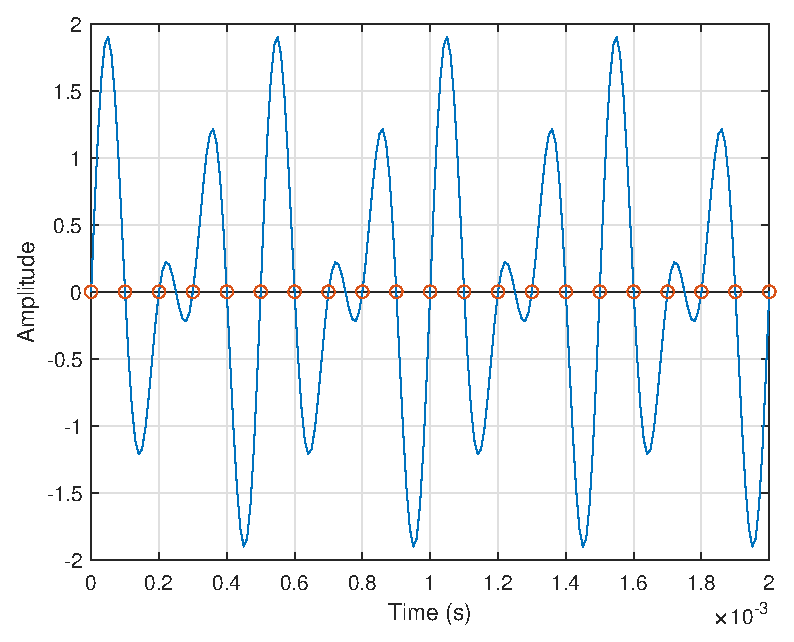
\includegraphics{fig/ex1_3.eps}
            \caption{Analogue (blue) and sampled (orange) signal.}
            \label{fig:ex1_3}
        \end{figure}
   \end{enumerate}
\end{exercise}

\begin{exercise}{Sampling 2}
    \begin{enumerate}
        \item See Figure \ref{fig:ex2_1}.
        \begin{figure}[h]
            \centering
            \begin{tikzpicture}
                \draw[->, very thick] (-3, 0) -- (3, 0) node[below]{$f$};
                \draw[->, very thick] (0, -2) -- (0, 2) node[above]{$X(f)$};

                \draw (-2.5, 0)node[below]{-5} -- (-2.5, 1.5);
                \draw(-2.5, 1.5) --node[above]{imag} (-0.5, 1.5);
                \draw(-0.5, 1.5) -- (0, 0);
                \draw(0, 0) -- (0.5, -1.5);
                \draw(0.5, -1.5) -- (2.5, -1.5);
                \draw(2.5, -1.5) -- (2.5, 0)node[above]{5};
            \end{tikzpicture}
            \caption{Sketch of imaginary and real parts of $X(f)$. (Real part is 0.)}
            \label{fig:ex2_1}
        \end{figure}
        \item See Figure \ref{fig:ex2_2}
        \begin{figure}[h]
            \centering
            \begin{tikzpicture}
                \draw[->, very thick] (-5, 0) -- (5, 0) node[below]{$f$};
                \draw[->, very thick] (0, -2) -- (0, 2) node[above]{$X(f)$};

                \draw(-4, 0)node[above]{$-8$} -- (-3.5, -1.5);
                \draw(-3.5, -1.5) -- (-1.5, -1.5);
                \draw(-1.5, -1.5) -- (-1.5, 0);

                \draw (-2.5, 0)node[below]{-5} -- (-2.5, 1.5);
                \draw(-2.5, 1.5) -- (-0.5, 1.5);
                \draw(-0.5, 1.5) -- (0, 0);
                \draw(0, 0) -- (0.5, -1.5);
                \draw(0.5, -1.5) -- (2.5, -1.5);
                \draw(2.5, -1.5) -- (2.5, 0)node[above]{5};

                \draw (1.5, 0) -- (1.5, 1.5);
                \draw(1.5, 1.5) -- (3.5, 1.5);
                \draw(3.5, 1.5) -- (4, 0)node[below]{$8$};

                \draw[dashed] (-2, -2.5) -- (-2, 2.5) node[above]{-4};
                \draw[dashed] (2, -2.5) -- (2, 2.5) node[above]{4};
                \draw[<->] (-2, -2.25) --node[below]{baseband} (2, -2.25);
            \end{tikzpicture}
            \caption{Sketch of the sprectrum of $x[n]$.}
            \label{fig:ex2_2}
        \end{figure}
    \end{enumerate}
\end{exercise}

\end{document}
